\subsection{Ghost particles}
\label{sss:aquagpusph:boundaries:ghostparticles}
%
`Ghost particles' is an algorithm so quite similar to `Fix particles' one, but in this case the extension of fluid
is not composed by particles linked to wall, that integrates their density using continuity equation, but is composed
by a mirroring of the fluid respect to the wall.\\
%
In the figure \ref{fig:aquagpusph:GhostParticlesScheme} a scheme about the fluid particles mirroring is shown.\\
%
So the SPH equation are therefore
%
\[
\left. \left\langle \frac{\gradient p}{\rho} \right\rangle_a \right\vert_{a \in \mathrm{Fluid}} = \frac{1}{\gamma_a}
	\sum\limits_{b \in \mathrm{Fluid}\;\cup\;\mathrm{Boundary}} 
		\left( \frac{p_a}{\rho_a^2} + \frac{p_b}{\rho_b^2} \right)
	\gradient W_{ab} m_b
\]
\[
\left. \left\langle \rho \; \divergence(v) \right\rangle_a \right\vert_{a \in \mathrm{Fluid}} =
	- \frac{1}{\gamma_a}
	\sum\limits_{b \in \mathrm{Fluid}\;\cup\;\mathrm{Boundary}} 
		\left( v_a - v_b \right)
	\gradient W_{ab} m_b
\]
\[
p_{a \in \mathrm{Boundary}} = \mathrm{f}\left(x_a, x_\mathrm{walls} \left( t \right) \right)
\]
\[
v_{a \in \mathrm{Boundary}} = \mathrm{f}\left(x_a, x_\mathrm{walls} \left( t \right) \right)
\]
%
The usual method to implement this boundary condition is perform a mirroring stage before the particles interaction,
storing the mirrored particles data in order to can use them within the fluid particles integration. In GPU
oriented code\footnote{and more generally for any parallel oriented one} this approach has the problem of the
previously unknown number of ghost particles, so memory reallocation or over-dimensioned arrays are mandatory
therefore. This can be walked around creating fix particles, but getting their values from fluid by a mirroring
operation and interpolation, with the advantage that the number of particles is ever know and reallocation is not
needed therefore, but with the disadvantage that requires to generate the fixed particles.\\
%
In \NAME a new algorithm is drafted, where the ghost particles are not precomputed, called `Virtual ghost particles'.
With this method a particles interaction process is called for each wall defined, so this method is not recommended
to high number of walls, nevertheless, when the particles interaction is called respect to a wall, each particle will
first test that is enough near to the wall before start working, so each `Ghost particles' interaction called is
significantly cheaper than usual one. The working method is locate all neighbours of the particle as is done on the
usual particles interaction method, and for each neighbour located compute the mirrored particle on runtime, avoiding
the need to store this data.\\
%
Since the number of walls must be relatively small, define the walls using particles with $imove < 0$ flag is not a
good option, so \NAME provides a parallel interface as has been described on chapter \ref{sss:XML:GhostParticles}.
This feature allows you to mix `Ghost particles' boundary condition with all other previous described, but probably
you only wants to mix it with `ElasticBounce boundary', in order to ensure than the fluid particles will not trespass
the walls.\\
%
`Ghost particles' boundary has the advantages of be easily defined in simple cases, and has been widely employed
along the SPH method history, so results can be easily compared. `Ghost particles' have some consistency problems
and is a condition bad defined in corners. When walls are perpendiculars the problem can be walked around adding
diagonal walls as shown in figure \ref{fig:aquagpusph:GhostParticlesCorner}, but for the moment general angles
intersection can not be solved in \NAME with `Ghost particles' boundary method yet.
%
\begin{figure}[h!]
  \centering
  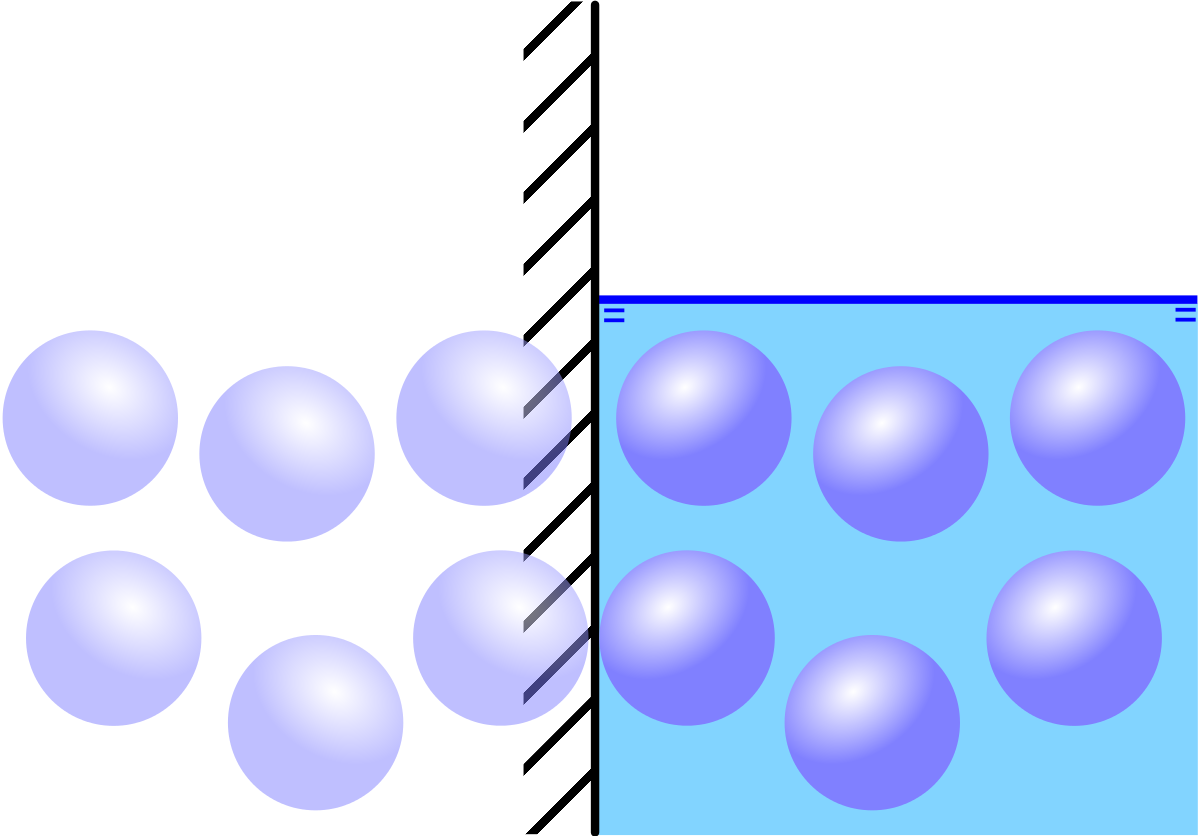
\includegraphics[width=0.4\textwidth]{GhostParticles}
  \caption{Ghost particles scheme}
  \label{fig:aquagpusph:GhostParticlesScheme}
\end{figure}
%
\begin{figure}[ht!]
  \centering
  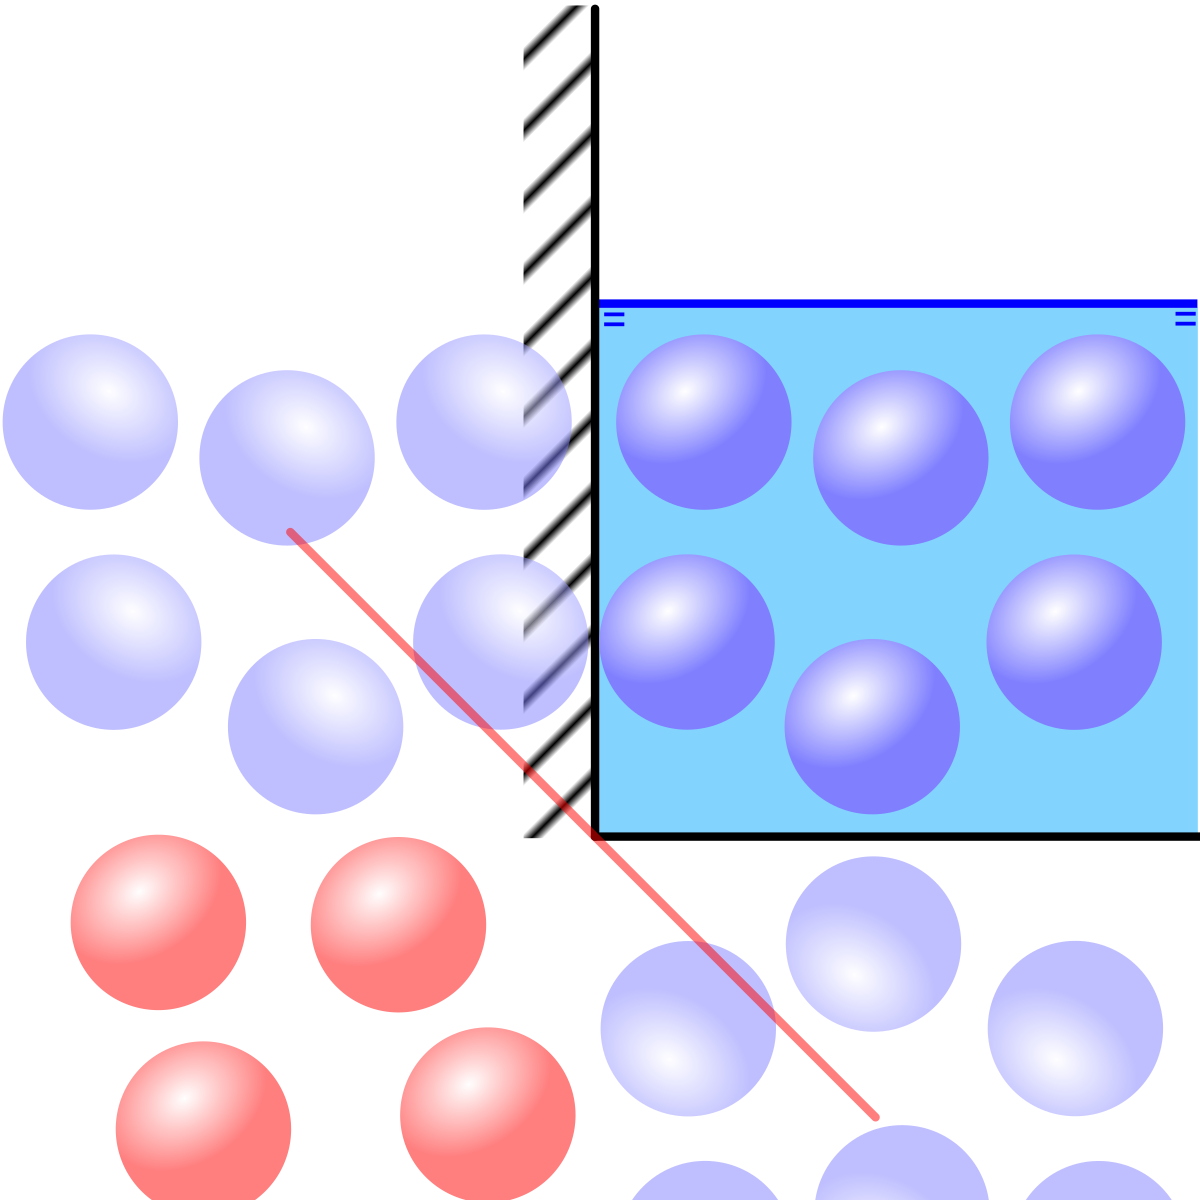
\includegraphics[width=0.4\textwidth]{GhostParticlesCorner}
  \caption{Ghost particles corner distribution}
  \label{fig:aquagpusph:GhostParticlesCorner}
\end{figure}
%
